\documentclass[manuscript,nonacm]{acmart}
%%
%% \BibTeX command to typeset BibTeX logo in the docs
\AtBeginDocument{%
  \providecommand\BibTeX{{%
    Bib\TeX}}}


\begin{document}

\title{Reimagining Transit Networks: A Data-Driven, Algorithmic Approach for the Washington DC Region}

\author{Spencer Jenkins}

\renewcommand{\shortauthors}{Trovato et al.}

\begin{abstract}
This paper presents a computational framework for the design of a reimagined rapid transit network for the Washington, DC metropolitan area. Motivated by the historical context and limitations of the existing WMATA system, my approach leverages geospatial analysis, graph algorithms, and data visualization to generate and evaluate alternative transit networks. The project consists of a transit network development pipeline, and a program to visualize and evaluate the generated networks. I describe the data sources, algorithms, and evaluation metrics used, and discuss the implications of my results for urban mobility and equity.
\end{abstract}

\maketitle



\section{Introduction}

This project was completed for CMSC 725: Geospatial Algorithms and Data, taught by Professor Hanan Samet.

Public transportation is a vital component of urban infrastructure, contributing to economic productivity~\cite{lit:us_transit_policy}, social equity~\cite{lit:equity}, and environmental sustainability~\cite{lit:us_transit_policy} in metropolitan areas. Washington, DC, and its surrounding areas in Maryland and Virginia, comprise the second-largest rapid transit network in the United States by daily ridership~\cite{lit:wmata_stats}. The network consists of six heavy rail lines spanning 208 kilometers and connecting 98 stations, operated by the Washington Metropolitan Area Transit Authority (WMATA)~\cite{lit:wmata_stats}. In 2019, the Washington Metro provided over 160 million trips per year, including work commutes, tourism, and other purposes~\cite{lit:wmata_stats}.

A primary goal in designing public transit networks in the U.S. is to reduce car dependency~\cite{lit:us_transit_policy}. However, the Washington Metro has struggled to achieve this, with only about 14\% of commuters in the region using transit~\cite{lit:commute_stats}. Comparable metropolitan areas such as Toronto report higher transit commute shares, while many European and Latin American cities also have significantly higher shares~\cite{lit:toronto}. These statistics are typically limited to work commutes, as data for other trip types is less available~\cite{lit:commute_stats}.

The limited success of the Washington Metro in attracting ridership is largely attributable to the priorities at the time of its planning~\cite{lit:wmata_history}. Unlike older East Coast cities with legacy rail systems, the Metro was conceived in the 1950s, an era of expanding car infrastructure and urban expressways. The Metro was designed as a compromise, connecting car commuters to the city center, with expansions primarily serving suburban areas~\cite{lit:wmata_history}. As a result, the network remains largely radial and focused on suburban commuters.

This design philosophy limits practical use. The network makes suburb-to-suburb and circumferential travel difficult, often requiring passengers to travel into the city center and transfer, even for short cross-town trips~\cite{lit:wmata_stats}. High-density neighborhoods such as Georgetown and marginalized areas like Anacostia have been historically underserved due to political, financial, and social factors~\cite{lit:equity}. Despite significant investment, the Metro has not achieved a substantial reduction in vehicle miles traveled (VMT) or car dependency~\cite{lit:env}. The static nature of the network has also hindered adaptation to shifting population centers and job clusters.

The persistent gaps in the current network's ability to connect high-density and underserved regions further motivate a new approach. For example, the lack of direct connections between major suburban job centers or marginalized neighborhoods limits economic opportunity and social inclusion~\cite{lit:equity}. Existing evaluation frameworks may overlook these gaps, focusing on aggregate metrics that mask disparities in access and service quality.

To address these challenges, this study combines computational and geospatial techniques to generate, evaluate, and visualize alternative transit networks for the Washington, DC region. This project leverages core concepts from CMSC 725, including spatial data structures (such as quadtrees and B-trees), proximity graphs, and efficient spatial querying, to address the challenges of transit network design. The methodology integrates geospatial analysis, graph algorithms, and data-driven optimization to generate and evaluate alternative transit networks for the Washington, DC region. By applying techniques from the course, such as kernel density estimation for spatial demand modeling and the use of Gabriel graphs for candidate network construction, the project demonstrates the power of computational geometry and geospatial algorithms in solving real-world urban problems~\cite{lit:spatial_algorithms}.


% --- Table: Counties and FIPS codes ---

% Table 1: Counties and County-Equivalents Considered

\begin{table}[h]
\caption{Counties and County-Equivalents in the Study Area}
\label{tab:counties}
\begin{tabular}{lccc}
\toprule
County/Equivalent & 2020 Population & Density (per km$^2$) & FIPS Code \\
\midrule
Prince George's & [value] & [value] & [value] \\
Montgomery & [value] & [value] & [value] \\
District of Columbia & [value] & [value] & [value] \\
Arlington County & [value] & [value] & [value] \\
Alexandria City & [value] & [value] & [value] \\
Falls Church City & [value] & [value] & [value] \\
Fairfax County & [value] & [value] & [value] \\
Fairfax City & [value] & [value] & [value] \\
Loudoun County & [value] & [value] & [value] \\
\bottomrule
\end{tabular}
\end{table}

% --- Table: Data Sources ---

\begin{table}[h]
\caption{Key Data Sources Used in the Study}
\label{tab:datasources}
\begin{tabular}{ll}
\toprule
Source & Description \\
\midrule
US Census Bureau & Census block population, shapefiles \\
Open Data DC/MD/VA & Points of interest, transit stops, land use \\
Arlington County & Neighborhood boundaries \\
State of Maryland & Neighborhood boundaries \\
District of Columbia & Neighborhood centroids \\
WMATA & Existing transit network \\
\bottomrule
\end{tabular}
\end{table}

% --- Figure: KDE Map ---

\begin{figure}[h]
    \centering
    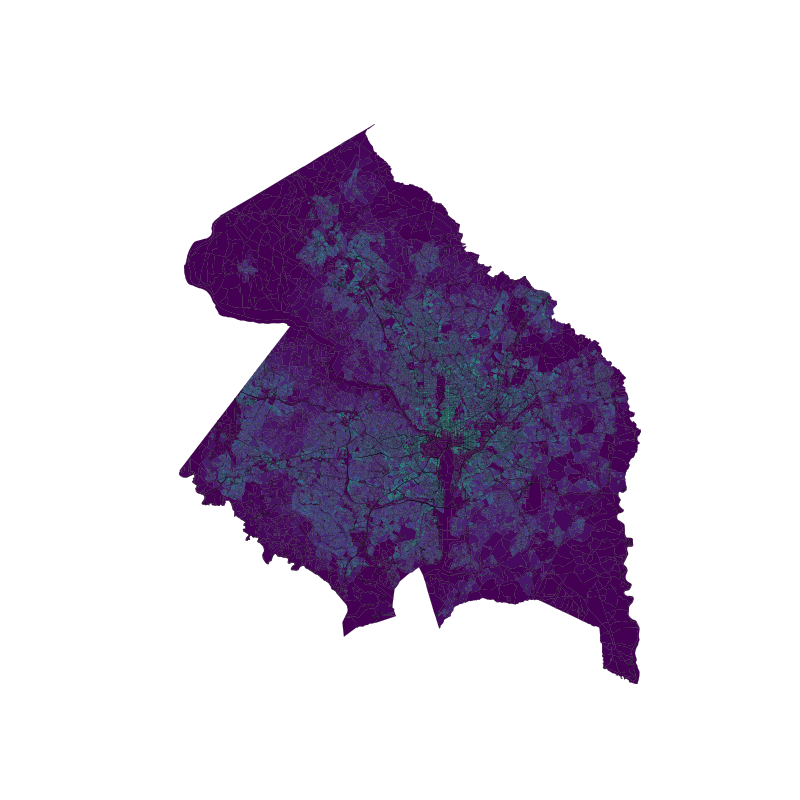
\includegraphics[width=0.7\textwidth]{img/transit_potential.png}
    \caption{Kernel density estimation (KDE) map of transit potential in the Washington, DC region.}
    \label{fig:kde}
\end{figure}

% --- Figure: Network Map Example ---

\begin{figure}[h]
    \centering
    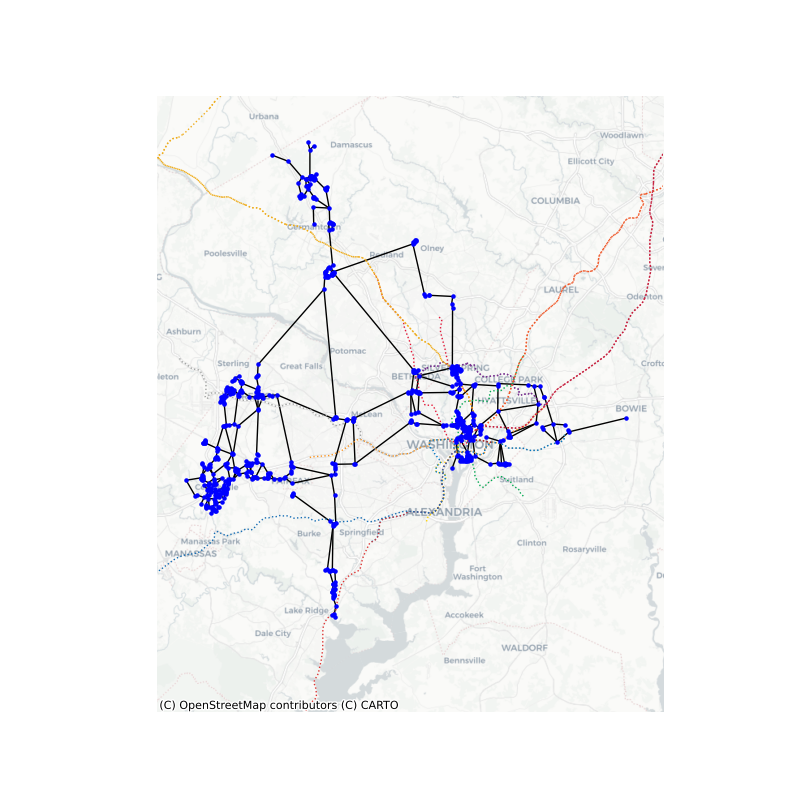
\includegraphics[width=0.7\textwidth]{img/network_map.png}
    \caption{Example of a generated candidate network overlaid on the metropolitan area.}
    \label{fig:networkmap}
\end{figure}

% --- Figure: Schematic Map Example ---

\begin{figure}[h]
    \centering
    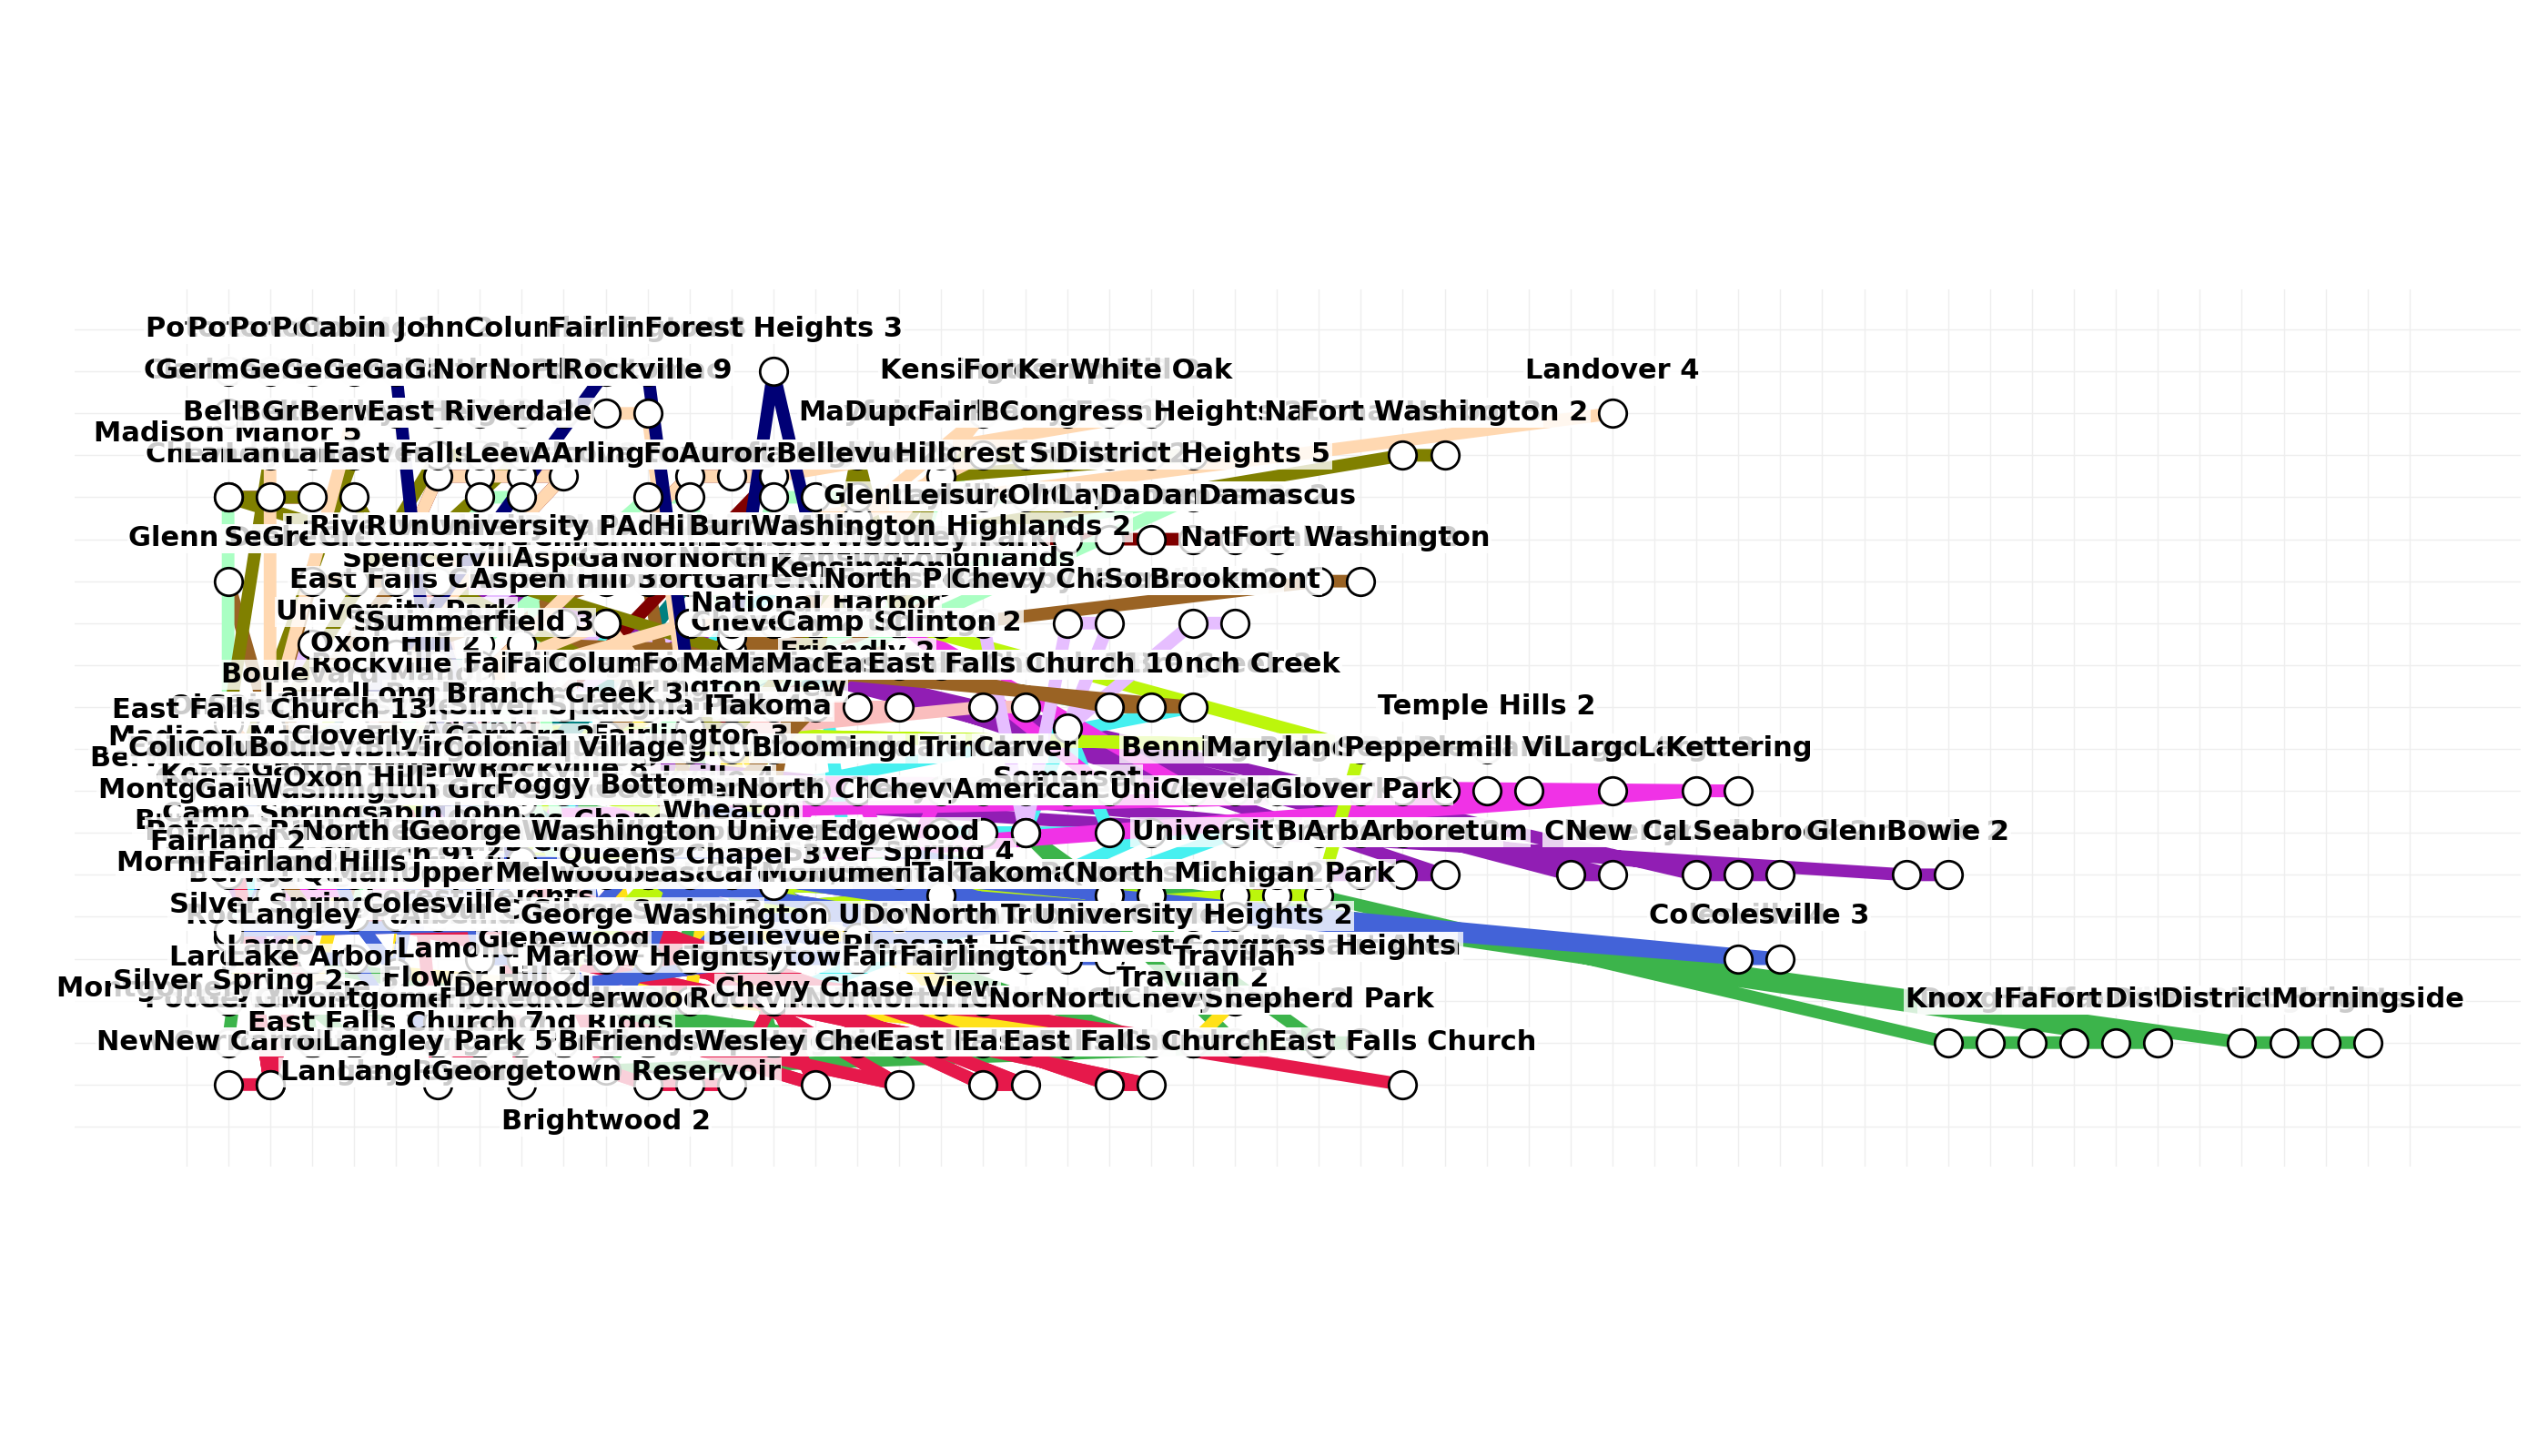
\includegraphics[width=0.7\textwidth]{img/lines_genetic.png}
    \caption{Schematic map of a generated network using the genetic algorithm.}
    \label{fig:schematic}
\end{figure}

\section{Network Design}

In this section, the network design process is detailed, including data collection, transformation, metric construction, network generation constraints, and the definition of the transit network search space. The network is built within this search space according to the scoring metrics and constraints, followed by post-processing.

\subsection{Data Sources and Transformation}
The first step is to define the study area. Table~\ref{tab:counties} lists the counties and county-equivalents included, along with their 2020 population, density, and FIPS code~\cite{lit:census}. Data for the Washington Metropolitan Area is available from Open Data DC, Open Data MD, and the Virginia Open Data Portal~\cite{lit:opendata}. Census block population data is obtained from the US Census Bureau. Transit potential for each block is calculated as population divided by area. A recursive spatial tree algorithm identifies the highest-need locations for transit, using a depth of 8. The resulting points represent locations with the highest need for transit based on population.

This data is augmented with points for important destinations, as shown in Table~\ref{tab:datasources}. The selection reflects the availability of data from each source. The study also includes all bus and rail stops in the counties listed, to approximate areas of high transit importance.

Raw data is transformed for network analysis using \texttt{geopandas}, with all data projected to a common CRS (typically EPSG:3857). Centroids are calculated for each census block and other points, providing candidate locations for potential stations. Unique identifiers and relevant attributes are assigned to each spatial unit. Intermediate results are saved as GeoJSON files for reproducibility and efficient reloading. This preprocessing pipeline, implemented in \texttt{eda.ipynb} and \texttt{funcs.py}, ensures the data is clean, consistent, and ready for network construction.

A kernel density estimate (KDE) is constructed over the selected points to provide scores for spatial queries at several stages. Figure~\ref{fig:kde} shows the KDE map for the area.

A mesh of candidate transit points is generated to balance spatial coverage with computational tractability. Population-based points (census block centroids) are combined with non-population points and deduplicated. The Gabriel graph, constructed using \texttt{libpysal.weights.Gabriel}, connects mutually closest points, resulting in a proximity network suitable for transit planning. The Gabriel graph is converted to a \texttt{networkx} graph for further manipulation, including assignment of edge weights based on Euclidean distance. This mesh serves as the substrate for both random walk and genetic algorithm-based network generation.

A Gabriel graph is constructed using the points. The graph is contracted by condensing Louvain communities by a user-defined threshold, forming the overall search space for the network. The network is constructed from the nodes and edges of this graph.

With the data fully preprocessed, one of three network construction algorithms is used to determine which line segments from the contracted Gabriel graph become part of the transit network.

% --- Figure: Contracted Gabriel Graph ---
Figure~\ref{fig:contractedgraph} shows the contracted Gabriel graph used as the search space for network generation.

\subsection{Network Creation: Naive (Random Walk) Algorithm}

The naive method involves constrained walks through the graph. Each walk starts from a random, previously unexplored node and follows the available edge leading to the greatest score. For each subsequent step, the walk chooses an available edge according to a weighted distribution: 75\% probability for the straightest angle, 25\% for the highest KDE score. Only edges forming at least a 130-degree angle from the previous edge can be chosen, and if the overall trajectory deviates by more than 80 degrees, the walk must proceed down edges that bring the angle back. If the walk reaches a node with no options, it terminates and attempts to continue from the original endpoint in the opposite direction. The walk is only kept if it is within a specified length range (45--100 km).

Edges are available if they are unexplored or have been explored up to three times. This reflects the interlined nature of the WMATA Metro, where several lines share alignments.

\subsection{Network Creation: Iterative Improvement Algorithm}

The iterative improvement method initializes a set of random walks. Walks are scored by the sum of KDE scores for all nodes, indicating transit utility. The lowest-scoring walk is replaced with a higher-scoring walk, and this process is repeated up to 100 times.

\subsection{Network Creation: Genetic Algorithm}
The genetic algorithm (GA) is a population-based metaheuristic inspired by natural selection. In this project, the GA optimizes rapid transit networks by evolving a population of candidate solutions toward higher fitness according to multiple criteria.

Each individual represents a candidate transit network, consisting of 20 lines, with a population size of 100. The initial population is generated by creating random sets of lines, as in the naive method. The fitness function evaluates how well a candidate network meets the objectives, as a weighted sum of:
\begin{itemize}
    \item \textbf{Demand Capture:} Sum of KDE scores for all nodes covered.
    \item \textbf{Coverage:} Rewards networks with more nodes (potential stations).
    \item \textbf{Pattern Bonus:} Rewards networks connecting suburban and dense areas.
    \item \textbf{Redundancy Penalty:} Penalizes networks for lines sharing alignments.
    \item \textbf{Load Penalty:} Penalizes networks with uneven service distribution.
    \item \textbf{Diversity Penalty:} Penalizes networks that are too similar within a generation.
\end{itemize}

Crossover and mutation produce the next generation. Crossover combines parts of two parent networks; mutation introduces random changes. Operators are designed to respect network constraints (valid paths, feasible line lengths). Elitism ensures the best individuals are retained. The algorithm runs for 30 generations, with efficient execution enabled by Python multiprocessing.

\subsection{Network Post-processing}
Each walk represents a candidate metro line. Lines are grouped by shared alignment using a pairwise distance matrix and a similarity threshold.

Not all nodes in the contracted Gabriel graph become stations due to varying edge lengths. Stations are selected as all terminal nodes, transfer points between different line groups, and nodes spaced at least 1 km apart. This ensures each station serves a catchment area of roughly 500 meters, corresponding to a 15-minute walk.

Station names are assigned by proximity to neighborhood centroids, using data from Arlington County, Maryland, and the District of Columbia. If multiple stations fall within the same neighborhood, a numeric suffix is added. I was unable to find neighborhood name or boundary data for for other parts of Virginia.

\subsection{Benchmarks and Evaluation Criteria}
Candidate networks are evaluated using benchmarks that reflect practical and theoretical priorities: geographic coverage (fraction of high-demand areas served), network connectivity (linking major regions), efficiency (minimizing redundant or excessively long lines), and demand capture (maximizing KDE-weighted coverage). These metrics are computed for each network and inform both random walk scoring and the genetic algorithm's fitness function.

\subsection{Influential Hyperparameters}
There were many hyperparameters that contributed to the success or lack thereof of the input. Table \ref{tab:hyperparams} shows the hyperparameters and the values used. The Louvain community resolution threshold was a key factor in determining the success of the network creation algorithm. Higher networks lead to stronger community contraction, leading to sparser graphs. The value of 0.07 provided a balance between a network with far too large of a search space and far too long considering short edges of less than a city block, while values that were too great resulted in suburban nodes being greatly reduced or lost. The line minimum and maximum distance were selected to reflect the size of the Washington metropolitan area and the distance of similar rapid transit services across the United States. The angle constraints were chosen so that the course of a given transit line would be preserved while still allowing for options and randomness. A minimum angle constraint of greater than 130 degrees results in premature halting of the walk algorithm as many nodes do not have any edges with angles greater than this. The same applies to the maximum deviation and maximum reset angles, where values too low for both hyperparameters results in walks reaching nodes they cannot proceed from. The station catchment area size, used in determining station scoring and spacing, is set to 500 meters, which reflects an average walking speed of 3 km/hr with Manhattan distance, and indicates the range around a station accessible by walking speed. The genetic algorithm weights were chosen to provide the strongest preference towards networks with coverage of low- and high-density areas on the same line. 

% --- Hyperparameter Table ---
\begin{table}[h]
\caption{Key Hyperparameters Used in Network Generation}
\label{tab:hyperparams}
\begin{tabular}{lll}
\toprule
\textbf{Hyperparameter} & \textbf{Explanation} & \textbf{Value} \\
\midrule
Louvain community resolution threshold & Controls granularity of community contraction & 0.07 \\
Line minimum distance & Minimum allowed length for a line (meters) & 45,000 \\
Line maximum distance & Maximum allowed length for a line (meters) & 100,000 \\
Minimum angle & Minimum angle between consecutive edges (degrees) & 130 \\
Maximum deviation angle & Angle leading to walk behavior forcing return to course & 80 \\
Maximum reset angle & Angle that will reset return-to-course behavior (degrees) & 30 \\
Group assignment threshold & Similarity threshold for grouping lines & 50\% \\
Station radius & Minimum distance between stations (meters) & 500 \\
Iterative improvement iterations & Number of iterations for improvement algorithm & 100 \\
Genetic: total score weight & Weight for total score in fitness function & 1 \\
Genetic: service pattern weight & Weight for service pattern in fitness function & 1000 \\
Genetic: redundancy penalty weight & Penalty for redundant lines in fitness function & -50 \\
Genetic: load penalty weight & Penalty for uneven service distribution & -20 \\
Genetic: diversity incentive weight & Incentive for diversity in population & -1 \\
\bottomrule
\end{tabular}
\end{table}

% --- Figure: Example Schematic Map ---
\begin{figure}[h]
    \centering
    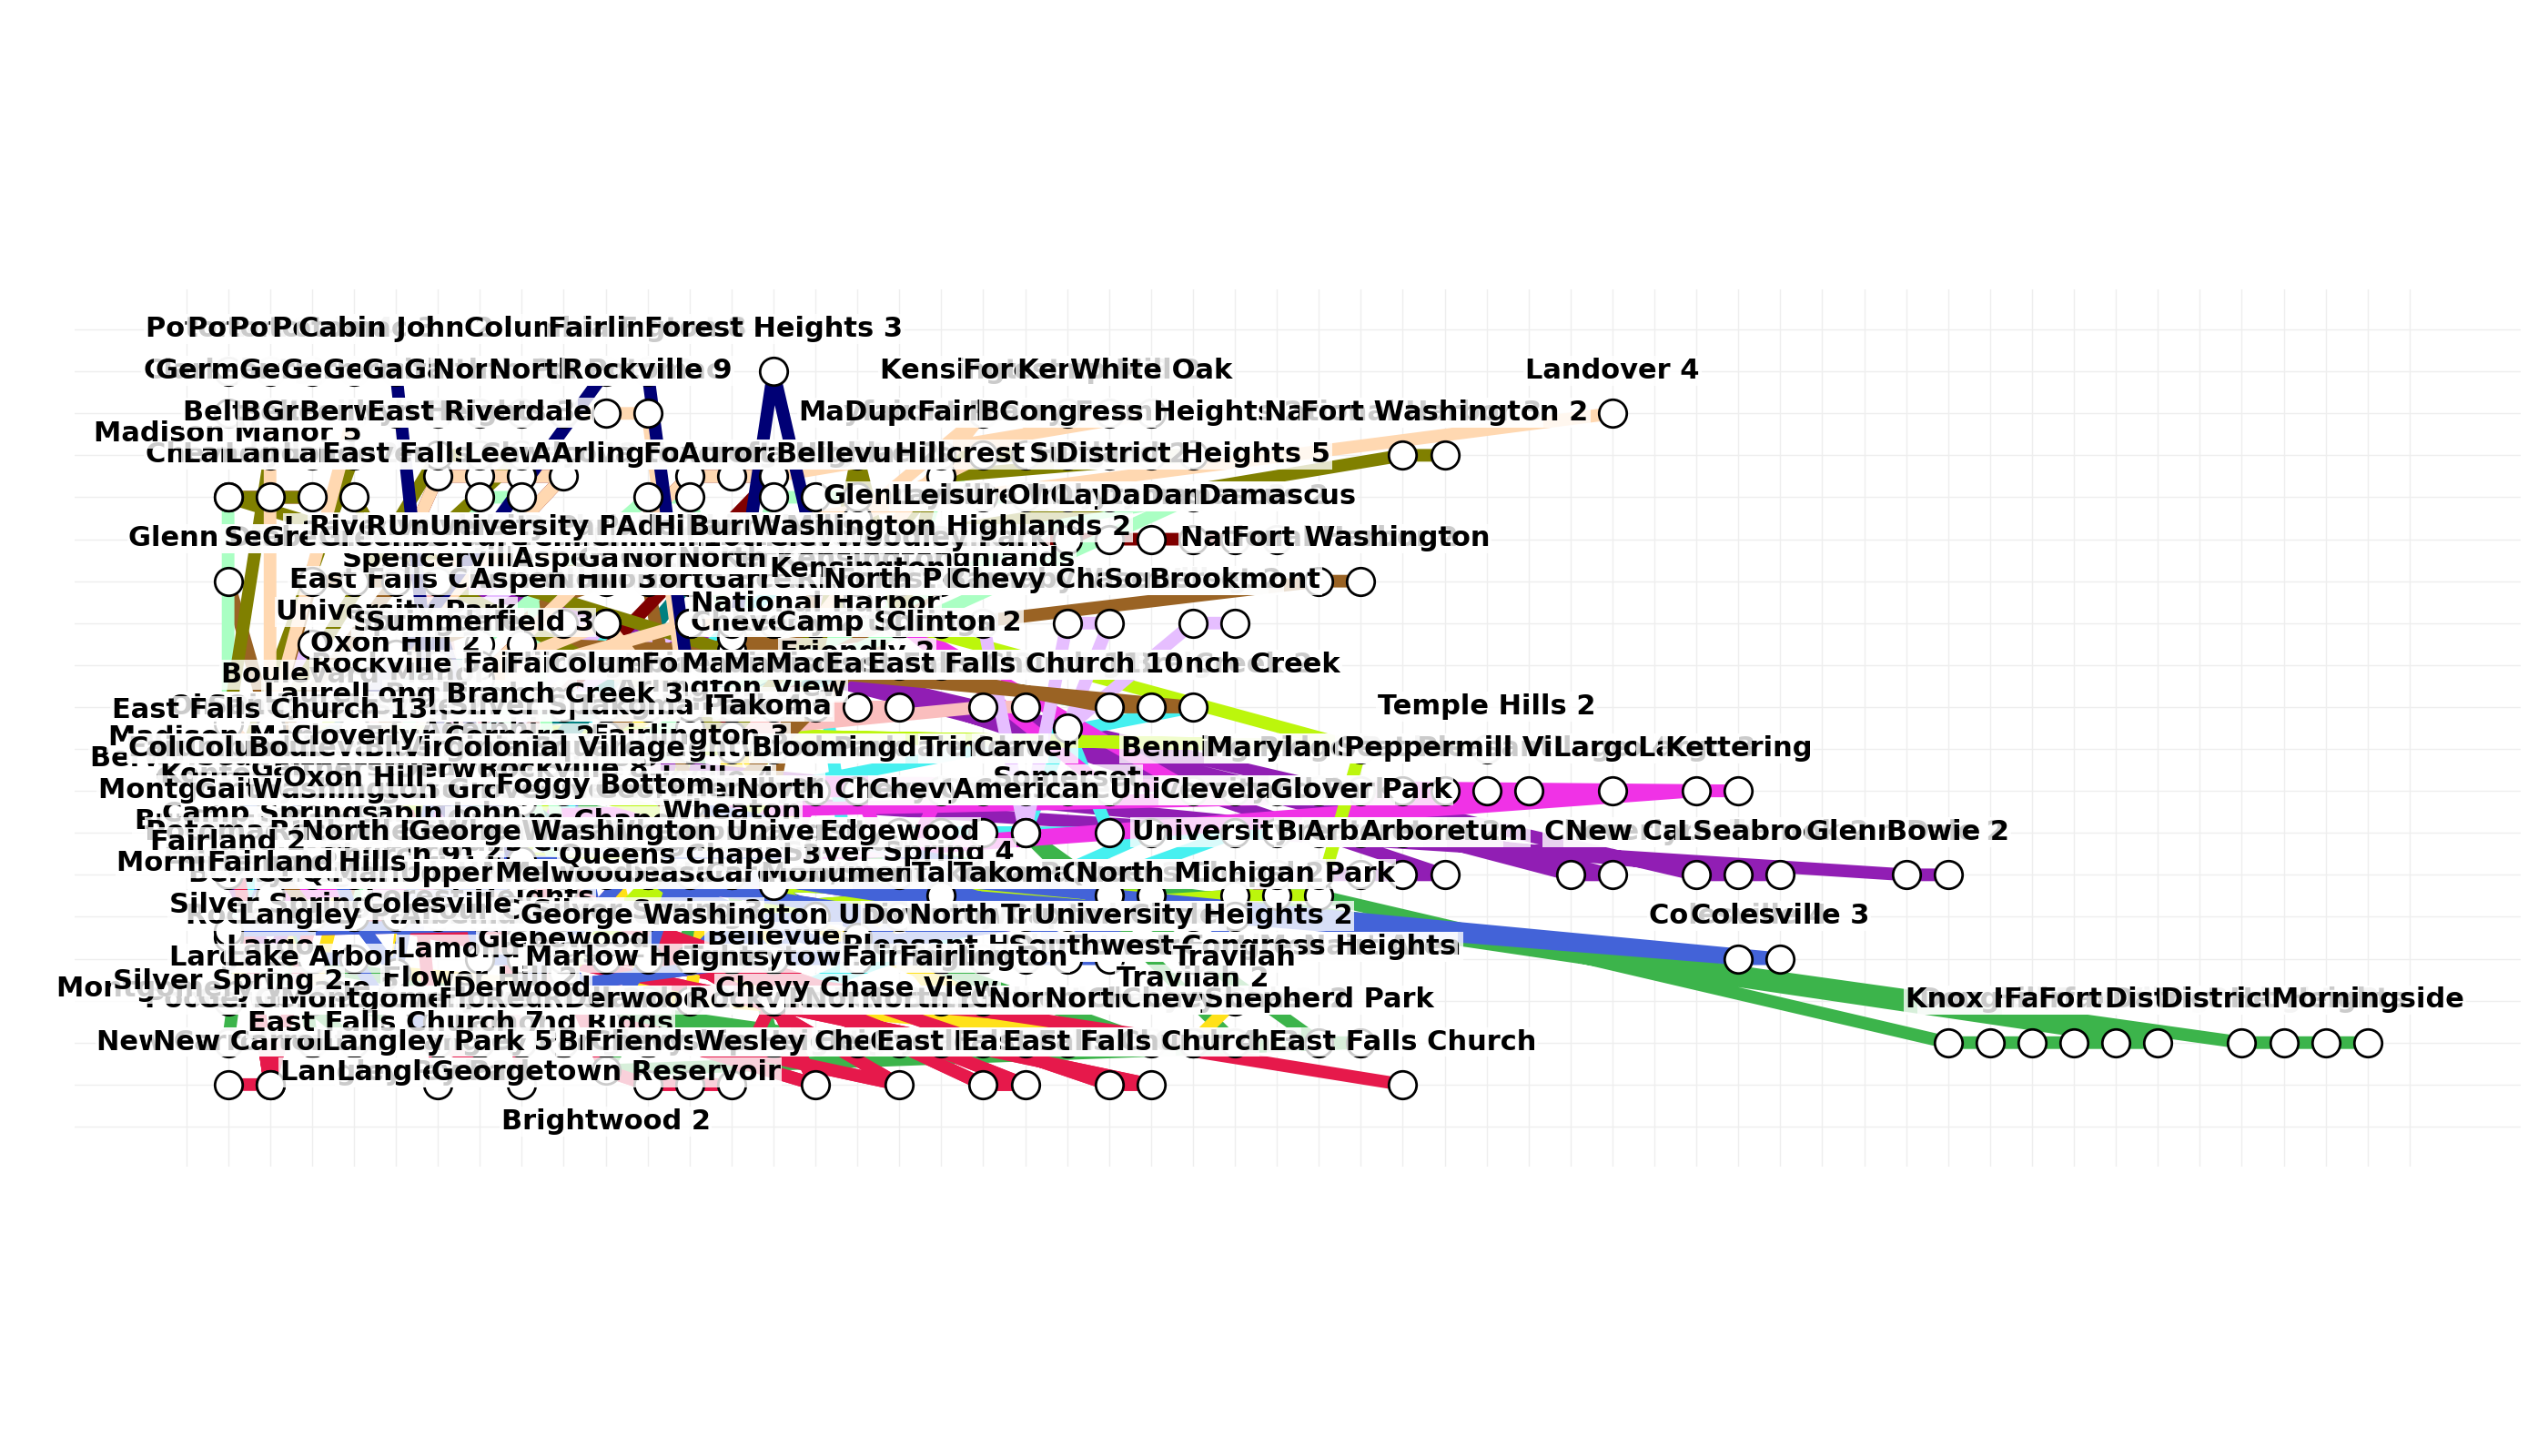
\includegraphics[width=0.7\textwidth]{img/lines_genetic.png}
    \caption{Schematic map of a generated network using the genetic algorithm.}
    \label{fig:schematic2}
\end{figure}

\section{Network Visualization and Exploration}

The Transit Network Viewer application, developed as a part of this project, allows users to visualize and explore the networks created using the algorithms designed in this project. The web application is highly interactive, allowing users to compare networks, examine specific lines, view station names, and determine estimated travel times. 

The web application's interface centers around a mapping tool powered by Leaflet. The interactive map displays the networks outputted by each of the three algorithms. Users can use checkboxes below the map to choose to view or hide specific lines, show the real-world transit network for comparison, view the catchment areas for each station, or view the contracted Gabriel graph used to generate the network. Users can hover over the transit lines, colored by group, to see helpful tooltips including their start and end locations, total distance, and number of stations. Users can hover the mouse over stations to see their name, lines served, and score. 

The most important feature of the Transit Network Viewer is the Route Finder, which users can use to calculate the travel time between selected start and end locations. The route is determined using Dijkstra's algorithm, with a penalty incurred for every time a route requires a transfer. If the user selects start and end locations that are not at stations, walking time estimates are included for the parts of the itinerary both before and after the trip through the metro network. If an itinerary is found, a window displays the details of the itinerary, including the route required, the number of stations the route passes through, the total distance traveled, and the estimated travel time. The travel time calculation uses an average speed across the network of 80 km/h, 6 minutes per transfer, and a walking speed of 5 km/h. 

\section{Network Performance Analysis}

I analyze the success of the networks quantitatively using several metrics. First, I determine the critical coverage percentage by calculating the proportion of critical transit points (high-density census blocks, critical services) that fall within the catchment area of any station in the network. The neighborhood coverage percentage is the fraction of neighborhood centroids within the catchment areas of at least one station. I also take the average distance from the nearest station across the entire metropolitan area and for the District of Columbia. Table \ref{tab:networkmetrics} provides the calculated data for the networks I created using each algorithm, and for the real-world WMATA network.

\begin{table}[h]
\caption{Comparison of Network Designs on Key Metrics}
\label{tab:networkmetrics}
\begin{tabular}{lcccc}
\toprule
\textbf{Network} & \textbf{\% Critical Coverage} & \textbf{\% Neighborhood Coverage} & \textbf{Avg. dist, regional} & \textbf{Avg. dist, DC} \\
\midrule
Genetic & 17.47 & 6.61 & 11.03 & 0.92 \\
Iterative & 24.12 & 4.96 & 11.19 & 1.67 \\
Naive & 18.95 & 3.99 & 10.86 & 1.59 \\
\midrule
Real-world & 13.39 & 3.03 & 14.94 & 1.59 \\
\bottomrule
\end{tabular}
\end{table}

By the metrics established in this table, the networks produced by all three algorithms outperform the real-world network. They exhibit higher critical coverage and neighborhood coverage rates, and provide lower average distances across the region. Each algorithm performs most strongly in a different metric: the genetic algorithm performs most strongly in neighborhood coverage and average distance within DC, while the naive algorithm shows the lowest average distance across the entire region, and the iterative improvement algorithm shows the highest critical coverage. 

I also perform some potential use-case evaluation by identifying location pairs and calculating the transit time in each network. I calculate the transit times for my network using my Route Planner tool, and I calculate transit times for the real-world network using the WMATA transit planner application. In this report I compare the results obtained for three sample itineraries chosen to demonstrate a variety of transit uses and to address the shortcomings of the existing WMATA network that I raised in the introduction. The three routes presented in this paper are: College Park to DCA Airport (suburb to important hub), downtown Bethesda to Reston Center (suburb to suburb), and Congress Heights to downtown Silver Spring (disadvantaged neighborhood to suburb). For all three routes, the algorithms developed in this project provide faster transit times than the real-world network, with each algorithm having stronger performance on different routes. Table \ref{tab:transittimes} shows the travel times calculated for each network. 

% --- Table: Sample Transit Times ---
\begin{table}[h]
\caption{Sample Transit Times for Selected Origin-Destination Pairs}
\label{tab:transittimes}
\begin{tabular}{lccc}
\toprule
\textbf{Network} & \textbf{College Park → DCA} & \textbf{Bethesda → Reston} & \textbf{Congress Heights → Silver Spring} \\
\midrule
Genetic & 29 min & 41 min & 30 min \\
Iterative & 37 min & 1 hr 1 min & 19 min \\
Naive & 32 min & 32 min & 17 min \\
\midrule
Real-world & 43 min & 1 hr 7 min & 41 min \\
\bottomrule
\end{tabular}
\end{table}

Visual comparison of the three obtained networks can provide additional justification and insight. The network has strong suburb-to-suburb connection, and also has a few strong connections in the urban core, but there are some large underserved areas. This is likely because the search space is simply too large to ensure that random walks will construct a network that covers it sufficiently. This likely explains its low performance in neighborhood coverage and average station distance within DC.

The iterative improvement algorithm takes the most time to execute, but provides a much more robust and connective network, especially in the urban core. The network has strong connections between suburbs and the urban core, but suburb-to-suburb connections are more limited. This is likely because the reward mechanism simply rewards routes with higher score sums for all stations across the line, so routes that gain a high increase in score due to being very long and travelling through DC are selected for. This likely explains its high critical coverage rate.

The genetic algorithm is the most sophisticated, and its output reflects this. There are strong connections between the urban core and suburbs in all directions, and coverage within the District of Columbia is strong as well. This is likely because of the service pattern reward weight, rewarding for routes that serve the urban core with connections to suburban areas. The high neighborhood coverage rate and low average distance within DC are likely due to this.

\subsection{Limitations}
The quality of the networks generated using my pipeline are only as good as the data they are created from. As discussed earlier, the data portals for each of the states varied wildly with respect to data depth and breadth. Virginia, in particular, did not have nearly as much data containing locations of areas supported by transit. Maryland and Washington, D.C. both had much more comprehensive data resources, which is expected given that Washington, D.C. is a single municipal jurisdiction and Maryland is a relatively small state mostly centered around a single metropolitan area. Virginia, on the other hand, is a large state with many metropolitan areas, and the data reflected this. There were often data of the sort I was interested in, but only for one or two counties and outside the DC area. 

The method of combining point data from multiple sources and creating a KDE from multiple sources entailed several limitations: first, each data point was treated as having the same transit importance, and the KDE therefore acted as a map of the amount of points in a given area. This means that the KDE scoring returned high values for regions that were well covered by the existing data, and low values for those with poor coverage, and no weight to whatever relative importance may have existed between points. The overall takeaway is that the transit algorithm happened to produce plausible-looking maps not as a reflection of the data, but because I constrained an otherwise random algorithm to produce results that look plausible. Across the three algorithms, I received wildly different results that often left many densely populated neighborhoods underserved. On the other hand, across algorithms, I obtained similar travel times between destination pairs, which is likely because with sufficient density, the network is large enough that one- or two-transfer routes on fairly straight alignments are possible between most urban destinations. It is also important to note that my network's reported high performance as compared to the real-world network is also likely largely attributable to the length and number of lines. Each algorithm produces a 20-line network, as compared to the real-world network which has six lines. 

In general, the method I have created in this project does not largely reflect the priorities or procedures of real-world transit agencies. Transit networks are not decided by random algorithms applied across entire metropolitan areas. The search space of the problem is still too great; there were not enough hard constraints on which areas the network should have connected. The result is a network that reaches most necessary areas because the number of randomly-generated lines is high enough. 

\subsection{Implications for Urban Transit Planning}
Despite the many shortcomings of the procedure inherent to this project, it still serves as a valuable tool at encouraging ambition and imagination in public transit planning. Although a 20-line metro system for the Washington metropolitan area would potentially cost hundreds of billions of dollars to construct, it would not be the first transit network of its size in the United States. The networks generated in this project are similar in density and robustness to the New York City Subway, which operates 28 service patterns across over 1000 km of track. New York City is far beyond all other American cities at reducing car usage, which is largely attributable to the coverage, speed, and dependability of its subway network. Although the New York metropolitan area is nearly three times as large as the Washington metropolitan area, the New York Subway does not expand beyond city limits into the suburbs, and the population within New York city limits of around 9 million is much more comparable to the population of the Washington metropolitan area. Therefore, a rapid transit network for the Washington metropolitan area that is significantly larger than the existing network would not be without comparison. 

\subsection{Future Work}

I hope to apply the general procedure of this work to create similar transit maps for other metropolitan areas in the United States. I also hope to explore deep learning-based approaches to learning a network, which I attempted but was unable to find a model that could converge on a non-trivial solution. 

\section{Acknowledgments}

I thank the instructors and peers of CMSC 725 for their feedback and support. I also acknowledge the open data providers, including the US Census Bureau, city- and state-level open data providers, and transit providers.

\bibliographystyle{ACM-Reference-Format}
\bibliography{sample-base}

\end{document}
